% Options for packages loaded elsewhere
\PassOptionsToPackage{unicode}{hyperref}
\PassOptionsToPackage{hyphens}{url}
\PassOptionsToPackage{dvipsnames,svgnames,x11names}{xcolor}
%
\documentclass[
  letterpaper,
  DIV=11,
  numbers=noendperiod]{scrartcl}

\usepackage{amsmath,amssymb}
\usepackage{iftex}
\ifPDFTeX
  \usepackage[T1]{fontenc}
  \usepackage[utf8]{inputenc}
  \usepackage{textcomp} % provide euro and other symbols
\else % if luatex or xetex
  \usepackage{unicode-math}
  \defaultfontfeatures{Scale=MatchLowercase}
  \defaultfontfeatures[\rmfamily]{Ligatures=TeX,Scale=1}
\fi
\usepackage{lmodern}
\ifPDFTeX\else  
    % xetex/luatex font selection
\fi
% Use upquote if available, for straight quotes in verbatim environments
\IfFileExists{upquote.sty}{\usepackage{upquote}}{}
\IfFileExists{microtype.sty}{% use microtype if available
  \usepackage[]{microtype}
  \UseMicrotypeSet[protrusion]{basicmath} % disable protrusion for tt fonts
}{}
\makeatletter
\@ifundefined{KOMAClassName}{% if non-KOMA class
  \IfFileExists{parskip.sty}{%
    \usepackage{parskip}
  }{% else
    \setlength{\parindent}{0pt}
    \setlength{\parskip}{6pt plus 2pt minus 1pt}}
}{% if KOMA class
  \KOMAoptions{parskip=half}}
\makeatother
\usepackage{xcolor}
\setlength{\emergencystretch}{3em} % prevent overfull lines
\setcounter{secnumdepth}{-\maxdimen} % remove section numbering
% Make \paragraph and \subparagraph free-standing
\makeatletter
\ifx\paragraph\undefined\else
  \let\oldparagraph\paragraph
  \renewcommand{\paragraph}{
    \@ifstar
      \xxxParagraphStar
      \xxxParagraphNoStar
  }
  \newcommand{\xxxParagraphStar}[1]{\oldparagraph*{#1}\mbox{}}
  \newcommand{\xxxParagraphNoStar}[1]{\oldparagraph{#1}\mbox{}}
\fi
\ifx\subparagraph\undefined\else
  \let\oldsubparagraph\subparagraph
  \renewcommand{\subparagraph}{
    \@ifstar
      \xxxSubParagraphStar
      \xxxSubParagraphNoStar
  }
  \newcommand{\xxxSubParagraphStar}[1]{\oldsubparagraph*{#1}\mbox{}}
  \newcommand{\xxxSubParagraphNoStar}[1]{\oldsubparagraph{#1}\mbox{}}
\fi
\makeatother

\usepackage{color}
\usepackage{fancyvrb}
\newcommand{\VerbBar}{|}
\newcommand{\VERB}{\Verb[commandchars=\\\{\}]}
\DefineVerbatimEnvironment{Highlighting}{Verbatim}{commandchars=\\\{\}}
% Add ',fontsize=\small' for more characters per line
\usepackage{framed}
\definecolor{shadecolor}{RGB}{241,243,245}
\newenvironment{Shaded}{\begin{snugshade}}{\end{snugshade}}
\newcommand{\AlertTok}[1]{\textcolor[rgb]{0.68,0.00,0.00}{#1}}
\newcommand{\AnnotationTok}[1]{\textcolor[rgb]{0.37,0.37,0.37}{#1}}
\newcommand{\AttributeTok}[1]{\textcolor[rgb]{0.40,0.45,0.13}{#1}}
\newcommand{\BaseNTok}[1]{\textcolor[rgb]{0.68,0.00,0.00}{#1}}
\newcommand{\BuiltInTok}[1]{\textcolor[rgb]{0.00,0.23,0.31}{#1}}
\newcommand{\CharTok}[1]{\textcolor[rgb]{0.13,0.47,0.30}{#1}}
\newcommand{\CommentTok}[1]{\textcolor[rgb]{0.37,0.37,0.37}{#1}}
\newcommand{\CommentVarTok}[1]{\textcolor[rgb]{0.37,0.37,0.37}{\textit{#1}}}
\newcommand{\ConstantTok}[1]{\textcolor[rgb]{0.56,0.35,0.01}{#1}}
\newcommand{\ControlFlowTok}[1]{\textcolor[rgb]{0.00,0.23,0.31}{\textbf{#1}}}
\newcommand{\DataTypeTok}[1]{\textcolor[rgb]{0.68,0.00,0.00}{#1}}
\newcommand{\DecValTok}[1]{\textcolor[rgb]{0.68,0.00,0.00}{#1}}
\newcommand{\DocumentationTok}[1]{\textcolor[rgb]{0.37,0.37,0.37}{\textit{#1}}}
\newcommand{\ErrorTok}[1]{\textcolor[rgb]{0.68,0.00,0.00}{#1}}
\newcommand{\ExtensionTok}[1]{\textcolor[rgb]{0.00,0.23,0.31}{#1}}
\newcommand{\FloatTok}[1]{\textcolor[rgb]{0.68,0.00,0.00}{#1}}
\newcommand{\FunctionTok}[1]{\textcolor[rgb]{0.28,0.35,0.67}{#1}}
\newcommand{\ImportTok}[1]{\textcolor[rgb]{0.00,0.46,0.62}{#1}}
\newcommand{\InformationTok}[1]{\textcolor[rgb]{0.37,0.37,0.37}{#1}}
\newcommand{\KeywordTok}[1]{\textcolor[rgb]{0.00,0.23,0.31}{\textbf{#1}}}
\newcommand{\NormalTok}[1]{\textcolor[rgb]{0.00,0.23,0.31}{#1}}
\newcommand{\OperatorTok}[1]{\textcolor[rgb]{0.37,0.37,0.37}{#1}}
\newcommand{\OtherTok}[1]{\textcolor[rgb]{0.00,0.23,0.31}{#1}}
\newcommand{\PreprocessorTok}[1]{\textcolor[rgb]{0.68,0.00,0.00}{#1}}
\newcommand{\RegionMarkerTok}[1]{\textcolor[rgb]{0.00,0.23,0.31}{#1}}
\newcommand{\SpecialCharTok}[1]{\textcolor[rgb]{0.37,0.37,0.37}{#1}}
\newcommand{\SpecialStringTok}[1]{\textcolor[rgb]{0.13,0.47,0.30}{#1}}
\newcommand{\StringTok}[1]{\textcolor[rgb]{0.13,0.47,0.30}{#1}}
\newcommand{\VariableTok}[1]{\textcolor[rgb]{0.07,0.07,0.07}{#1}}
\newcommand{\VerbatimStringTok}[1]{\textcolor[rgb]{0.13,0.47,0.30}{#1}}
\newcommand{\WarningTok}[1]{\textcolor[rgb]{0.37,0.37,0.37}{\textit{#1}}}

\providecommand{\tightlist}{%
  \setlength{\itemsep}{0pt}\setlength{\parskip}{0pt}}\usepackage{longtable,booktabs,array}
\usepackage{calc} % for calculating minipage widths
% Correct order of tables after \paragraph or \subparagraph
\usepackage{etoolbox}
\makeatletter
\patchcmd\longtable{\par}{\if@noskipsec\mbox{}\fi\par}{}{}
\makeatother
% Allow footnotes in longtable head/foot
\IfFileExists{footnotehyper.sty}{\usepackage{footnotehyper}}{\usepackage{footnote}}
\makesavenoteenv{longtable}
\usepackage{graphicx}
\makeatletter
\def\maxwidth{\ifdim\Gin@nat@width>\linewidth\linewidth\else\Gin@nat@width\fi}
\def\maxheight{\ifdim\Gin@nat@height>\textheight\textheight\else\Gin@nat@height\fi}
\makeatother
% Scale images if necessary, so that they will not overflow the page
% margins by default, and it is still possible to overwrite the defaults
% using explicit options in \includegraphics[width, height, ...]{}
\setkeys{Gin}{width=\maxwidth,height=\maxheight,keepaspectratio}
% Set default figure placement to htbp
\makeatletter
\def\fps@figure{htbp}
\makeatother

\usepackage{fvextra}
\DefineVerbatimEnvironment{Highlighting}{Verbatim}{breaklines,commandchars=\\\{\}}
\KOMAoption{captions}{tableheading}
\makeatletter
\@ifpackageloaded{caption}{}{\usepackage{caption}}
\AtBeginDocument{%
\ifdefined\contentsname
  \renewcommand*\contentsname{Table of contents}
\else
  \newcommand\contentsname{Table of contents}
\fi
\ifdefined\listfigurename
  \renewcommand*\listfigurename{List of Figures}
\else
  \newcommand\listfigurename{List of Figures}
\fi
\ifdefined\listtablename
  \renewcommand*\listtablename{List of Tables}
\else
  \newcommand\listtablename{List of Tables}
\fi
\ifdefined\figurename
  \renewcommand*\figurename{Figure}
\else
  \newcommand\figurename{Figure}
\fi
\ifdefined\tablename
  \renewcommand*\tablename{Table}
\else
  \newcommand\tablename{Table}
\fi
}
\@ifpackageloaded{float}{}{\usepackage{float}}
\floatstyle{ruled}
\@ifundefined{c@chapter}{\newfloat{codelisting}{h}{lop}}{\newfloat{codelisting}{h}{lop}[chapter]}
\floatname{codelisting}{Listing}
\newcommand*\listoflistings{\listof{codelisting}{List of Listings}}
\makeatother
\makeatletter
\makeatother
\makeatletter
\@ifpackageloaded{caption}{}{\usepackage{caption}}
\@ifpackageloaded{subcaption}{}{\usepackage{subcaption}}
\makeatother

\ifLuaTeX
  \usepackage{selnolig}  % disable illegal ligatures
\fi
\usepackage{bookmark}

\IfFileExists{xurl.sty}{\usepackage{xurl}}{} % add URL line breaks if available
\urlstyle{same} % disable monospaced font for URLs
\hypersetup{
  pdftitle={BST 270: Individual Project},
  pdfauthor={Shanta Murthy},
  colorlinks=true,
  linkcolor={blue},
  filecolor={Maroon},
  citecolor={Blue},
  urlcolor={Blue},
  pdfcreator={LaTeX via pandoc}}


\title{BST 270: Individual Project}
\usepackage{etoolbox}
\makeatletter
\providecommand{\subtitle}[1]{% add subtitle to \maketitle
  \apptocmd{\@title}{\par {\large #1 \par}}{}{}
}
\makeatother
\subtitle{Reproducible Data Science: Police Settlements
(FiveThirtyEight)}
\author{Shanta Murthy}
\date{}

\begin{document}
\maketitle


Here we will be using an \href{http://rmarkdown.rstudio.com}{R Markdown}
Notebook. When you execute code within the notebook, the results appear
beneath the code.

The article we will attempt to reproduce the results from is titled
\href{'\%20https://fivethirtyeight.com/features/police-misconduct-costs-cities-millions-every-year-but-thats-where-the-accountability-ends/'}{Cities
Spend Millions On Police Misconduct Every Year. Here's Why It's So
Difficult to Hold Departments Accountable}.

The article has a corresponding data and code available for
preprocessing which was used for reproducing select figures shown here,
accessible on the corresponding
\href{'https://github.com/fivethirtyeight/police-settlements/'}{original
GitHub}

Additionally, multiple levels of the processed files and separate codes
for preprocessing steps that were conducted were provided for each
city's data separately, including explanations of how the data was
formatted and cleaned with respect to the available data for each
location.

Sample outputs are provided in the output folder and the knitted file is
contained in the parent directory.

\subsection{Step 0. Load libraries, install if not already
loaded}\label{step-0.-load-libraries-install-if-not-already-loaded}

The packages that have been loaded are listed below and the
sessionInfo() at the bottom of this document (in the Appendix) provides
the version information for each of the packages. If any of these
packages have not already been installed, please install first using
install.packages() and then load the library with library() before
proceeding.

\subsection{Step 1. Load corresponding data files for all the following
figures.}\label{step-1.-load-corresponding-data-files-for-all-the-following-figures.}

We will attempt to reproduce the barplot of the Cleveland settlement
following Rice's death (``Figure 1''), comparison of misleading
categorization between Cincinnati and Charleston (``Figure 2''), and
Large settlements can skew a city's average payment (``Figure 3'')) from
the original FiveThirtyEight article on police settlements.

First, we will load the data files that have been provided in the
corresponding
\href{'https://github.com/fivethirtyeight/police-settlements/'}{FiveThirtyEight
GitHub}.

\begin{Shaded}
\begin{Highlighting}[]
\CommentTok{\# For Figure 1 {-} intermediate file from Cleveland Police Department dataset, can be loaded as follows (with respect to this folder, this is where we have stored the intermediate file)}
\NormalTok{intermediate\_cleveland }\OtherTok{\textless{}{-}}\NormalTok{ readxl}\SpecialCharTok{::}\FunctionTok{read\_xlsx}\NormalTok{(here}\SpecialCharTok{::}\FunctionTok{here}\NormalTok{(}\StringTok{\textquotesingle{}data/intermediate/clevelandstart.xlsx\textquotesingle{}}\NormalTok{))}

\CommentTok{\#For Figures 2 and 3 {-} load each of the final data files from GitHub page.}
\CommentTok{\# Define a list of cities with their respective paths and labels}
\NormalTok{city\_info }\OtherTok{\textless{}{-}} \FunctionTok{list}\NormalTok{(}
  \AttributeTok{springfield     =} \FunctionTok{c}\NormalTok{(}\StringTok{"springfield\_edited.csv"}\NormalTok{, }\StringTok{"Springfield, MA"}\NormalTok{),}
  \AttributeTok{milwaukee       =} \FunctionTok{c}\NormalTok{(}\StringTok{"milwaukee\_edited.csv"}\NormalTok{, }\StringTok{"Milwaukee"}\NormalTok{),}
  \AttributeTok{los\_angeles     =} \FunctionTok{c}\NormalTok{(}\StringTok{"los\_angeles\_edited.csv"}\NormalTok{, }\StringTok{"Los Angeles"}\NormalTok{),}
  \AttributeTok{san\_francisco   =} \FunctionTok{c}\NormalTok{(}\StringTok{"san\_francisco\_edited.csv"}\NormalTok{, }\StringTok{"San Francisco"}\NormalTok{),}
  \AttributeTok{washington\_dc   =} \FunctionTok{c}\NormalTok{(}\StringTok{"DC\_edited.csv"}\NormalTok{, }\StringTok{"Washington, D.C."}\NormalTok{),}
  \AttributeTok{chicago         =} \FunctionTok{c}\NormalTok{(}\StringTok{"chicago\_edited.csv"}\NormalTok{, }\StringTok{"Chicago"}\NormalTok{),}
  \AttributeTok{st\_louis        =} \FunctionTok{c}\NormalTok{(}\StringTok{"stlouis\_edited.csv"}\NormalTok{, }\StringTok{"St. Louis"}\NormalTok{),}
  \AttributeTok{baltimore       =} \FunctionTok{c}\NormalTok{(}\StringTok{"baltimore\_edited.csv"}\NormalTok{, }\StringTok{"Baltimore"}\NormalTok{),}
  \AttributeTok{boston          =} \FunctionTok{c}\NormalTok{(}\StringTok{"boston\_edited.csv"}\NormalTok{, }\StringTok{"Boston"}\NormalTok{),}
  \AttributeTok{cleveland       =} \FunctionTok{c}\NormalTok{(}\StringTok{"cleveland\_edited.csv"}\NormalTok{, }\StringTok{"Cleveland"}\NormalTok{),}
  \AttributeTok{little\_rock     =} \FunctionTok{c}\NormalTok{(}\StringTok{"little\_rock\_edited.csv"}\NormalTok{, }\StringTok{"Little Rock"}\NormalTok{),}
  \AttributeTok{new\_orleans     =} \FunctionTok{c}\NormalTok{(}\StringTok{"new\_orleans\_edited.csv"}\NormalTok{, }\StringTok{"New Orleans"}\NormalTok{),}
  \AttributeTok{waterbury       =} \FunctionTok{c}\NormalTok{(}\StringTok{"waterbury\_edited.csv"}\NormalTok{, }\StringTok{"Waterbury, CT"}\NormalTok{),}
  \AttributeTok{detroit         =} \FunctionTok{c}\NormalTok{(}\StringTok{"detroit\_edited.csv"}\NormalTok{, }\StringTok{"Detroit"}\NormalTok{),}
  \AttributeTok{orlando         =} \FunctionTok{c}\NormalTok{(}\StringTok{"orlando\_edited.csv"}\NormalTok{, }\StringTok{"Orlando"}\NormalTok{),}
  \AttributeTok{miami           =} \FunctionTok{c}\NormalTok{(}\StringTok{"miami\_edited.csv"}\NormalTok{, }\StringTok{"Miami"}\NormalTok{),}
  \AttributeTok{paterson        =} \FunctionTok{c}\NormalTok{(}\StringTok{"paterson\_edited.csv"}\NormalTok{, }\StringTok{"Paterson, NJ"}\NormalTok{),}
  \AttributeTok{atlanta         =} \FunctionTok{c}\NormalTok{(}\StringTok{"atlanta\_edited.csv"}\NormalTok{, }\StringTok{"Atlanta"}\NormalTok{),}
  \AttributeTok{philadelphia    =} \FunctionTok{c}\NormalTok{(}\StringTok{"philly\_edited.csv"}\NormalTok{, }\StringTok{"Philadelphia"}\NormalTok{),}
  \AttributeTok{baton\_rouge     =} \FunctionTok{c}\NormalTok{(}\StringTok{"baton\_rouge\_edited.csv"}\NormalTok{, }\StringTok{"Baton Rouge"}\NormalTok{),}
  \AttributeTok{indianapolis    =} \FunctionTok{c}\NormalTok{(}\StringTok{"indianapolis\_edited.csv"}\NormalTok{, }\StringTok{"Indianapolis"}\NormalTok{),}
  \AttributeTok{nyc             =} \FunctionTok{c}\NormalTok{(}\StringTok{"new\_york\_edited.csv"}\NormalTok{, }\StringTok{"New York City"}\NormalTok{),}
  \AttributeTok{cincinnati      =} \FunctionTok{c}\NormalTok{(}\StringTok{"cincinnati\_edited.csv"}\NormalTok{, }\StringTok{"Cincinnati"}\NormalTok{),}
  \AttributeTok{columbia        =} \FunctionTok{c}\NormalTok{(}\StringTok{"columbia\_edited.csv"}\NormalTok{, }\StringTok{"Columbia"}\NormalTok{),}
  \AttributeTok{north\_charleston=} \FunctionTok{c}\NormalTok{(}\StringTok{"north\_charleston\_edited.csv"}\NormalTok{, }\StringTok{"North Charleston, SC"}\NormalTok{),}
  \AttributeTok{charleston      =} \FunctionTok{c}\NormalTok{(}\StringTok{"charleston\_edited.csv"}\NormalTok{, }\StringTok{"Charleston, SC"}\NormalTok{),}
  \AttributeTok{memphis         =} \FunctionTok{c}\NormalTok{(}\StringTok{"memphis\_edited.csv"}\NormalTok{, }\StringTok{"Memphis, TN"}\NormalTok{),}
  \AttributeTok{fort\_lauderdale =} \FunctionTok{c}\NormalTok{(}\StringTok{"fort\_lauderdale\_edited.csv"}\NormalTok{, }\StringTok{"Fort Lauderdale, FL"}\NormalTok{),}
  \AttributeTok{roanoke         =} \FunctionTok{c}\NormalTok{(}\StringTok{"roanoke\_edited.csv"}\NormalTok{, }\StringTok{"Roanoke, VA"}\NormalTok{),}
  \AttributeTok{cambridge       =} \FunctionTok{c}\NormalTok{(}\StringTok{"cambridge\_edited.csv"}\NormalTok{, }\StringTok{"Cambridge, MA"}\NormalTok{),}
  \AttributeTok{richmond        =} \FunctionTok{c}\NormalTok{(}\StringTok{"richmond\_edited.csv"}\NormalTok{, }\StringTok{"Richmond, VA"}\NormalTok{)}
\NormalTok{)}

\CommentTok{\# Create an empty list to store data}
\NormalTok{city\_datasets }\OtherTok{\textless{}{-}} \FunctionTok{list}\NormalTok{()}

\CommentTok{\# Save out file name and lab}
\ControlFlowTok{for}\NormalTok{ (city }\ControlFlowTok{in} \FunctionTok{names}\NormalTok{(city\_info)) \{}
\NormalTok{  filename }\OtherTok{\textless{}{-}}\NormalTok{ city\_info[[city]][}\DecValTok{1}\NormalTok{]}
\NormalTok{  label }\OtherTok{\textless{}{-}}\NormalTok{ city\_info[[city]][}\DecValTok{2}\NormalTok{]}
  
  \CommentTok{\# Read and mutate final, processed data (stored in processed folder) to name city\_label for column}
\NormalTok{  city\_datasets[[city]] }\OtherTok{\textless{}{-}} \FunctionTok{read.csv}\NormalTok{(here}\SpecialCharTok{::}\FunctionTok{here}\NormalTok{(}\StringTok{"data/processed"}\NormalTok{, filename)) }\SpecialCharTok{\%\textgreater{}\%}
    \FunctionTok{mutate}\NormalTok{(}\AttributeTok{city\_label =}\NormalTok{ label)}
\NormalTok{\}}

\CommentTok{\# Assign each dataset to a variable {-} this will create a variable of each city name separately which will be used in Figure 2 and Figure 3 generation}
\ControlFlowTok{for}\NormalTok{ (city }\ControlFlowTok{in} \FunctionTok{names}\NormalTok{(city\_datasets)) \{}
  \FunctionTok{assign}\NormalTok{(city, city\_datasets[[city]])}
\NormalTok{\}}

\CommentTok{\#These are now stored according to their respective city.}
\end{Highlighting}
\end{Shaded}

\subsection{Step 2. Figure 1: `Cleveland's settlement amounts rose after
Rice's
death'}\label{step-2.-figure-1-clevelands-settlement-amounts-rose-after-rices-death}

Using intermediate data file corresponding to the Cleveland dataset, we
are able to conduct the preprocessing steps described in
\href{'https://github.com/fivethirtyeight/police-settlements/blob/main/cleveland_oh/cleveland_oh.R'}{cleveland\_oh.R}
corresponding script with function to generate plot. As the
\href{'https://github.com/fivethirtyeight/police-settlements/blob/main/cleveland_oh/README.md'}{original
GitHub} states, they were provided settlement data for cases paid out
between 2010 and 2020. In this calendar year corresponds to the year the
settlement was paid out and there was no information regarding the type
of misconduct, so this was not used in the filtering process. The
authors stated that while some cases included settlements that were paid
out in multiple installments over more than 1 year, the data has been
defined as amount Cleveland paid per year rather than the number of
cases settled in each year. The preprocessing steps have been copied
into the script sourced below, and we were able to conduct the same
preprocessing and get the same final outputs using the checks provided
in the original script. Thus the preprocessing steps appear to be
consistent with those that the authors had used. We have additionally
added the steps for visualizing the data which was not provided in the
published FiveThirtyEight script, and visualize it below.

\begin{Shaded}
\begin{Highlighting}[]
\CommentTok{\#Use intermediate\_cleveland file to process data appropriately (described in corresponding R script)}
\FunctionTok{source}\NormalTok{(here}\SpecialCharTok{::}\FunctionTok{here}\NormalTok{(}\StringTok{\textquotesingle{}helper\_functions/Figure1\_policesettlements.R\textquotesingle{}}\NormalTok{))}

\CommentTok{\#Visualize figure 1 plot }

\NormalTok{F1 }\OtherTok{\textless{}{-}} \FunctionTok{figure1}\NormalTok{(intermediate\_cleveland)}
\end{Highlighting}
\end{Shaded}

\begin{verbatim}
[1] "There are 142 rows missing closed date"
[1] "There are 0 rows missing calendar year"
[1] "There are 0 rows missing amount awarded"
[1] "There are 0 rows with amount awarded = 0"
[1] "There are 0 rows missing docket number"
[1] "Total number of cases"
[1] 142
[1] "Total amount awarded"
\end{verbatim}

\begin{Shaded}
\begin{Highlighting}[]
\FunctionTok{ggsave}\NormalTok{(}\AttributeTok{filename =}\NormalTok{ here}\SpecialCharTok{::}\FunctionTok{here}\NormalTok{(}\StringTok{\textquotesingle{}plots/\textquotesingle{}}\NormalTok{, }\StringTok{"Figure1\_output.png"}\NormalTok{), }
       \AttributeTok{plot =}\NormalTok{ F1, }
       \AttributeTok{bg =} \StringTok{"white"}\NormalTok{, }\AttributeTok{width =} \DecValTok{10}\NormalTok{, }\AttributeTok{height =} \FloatTok{6.5}\NormalTok{, }\AttributeTok{units =} \StringTok{"in"}\NormalTok{)}
\NormalTok{knitr}\SpecialCharTok{::}\FunctionTok{include\_graphics}\NormalTok{(here}\SpecialCharTok{::}\FunctionTok{here}\NormalTok{(}\StringTok{"plots"}\NormalTok{, }\StringTok{"Figure1\_output.png"}\NormalTok{))}
\end{Highlighting}
\end{Shaded}

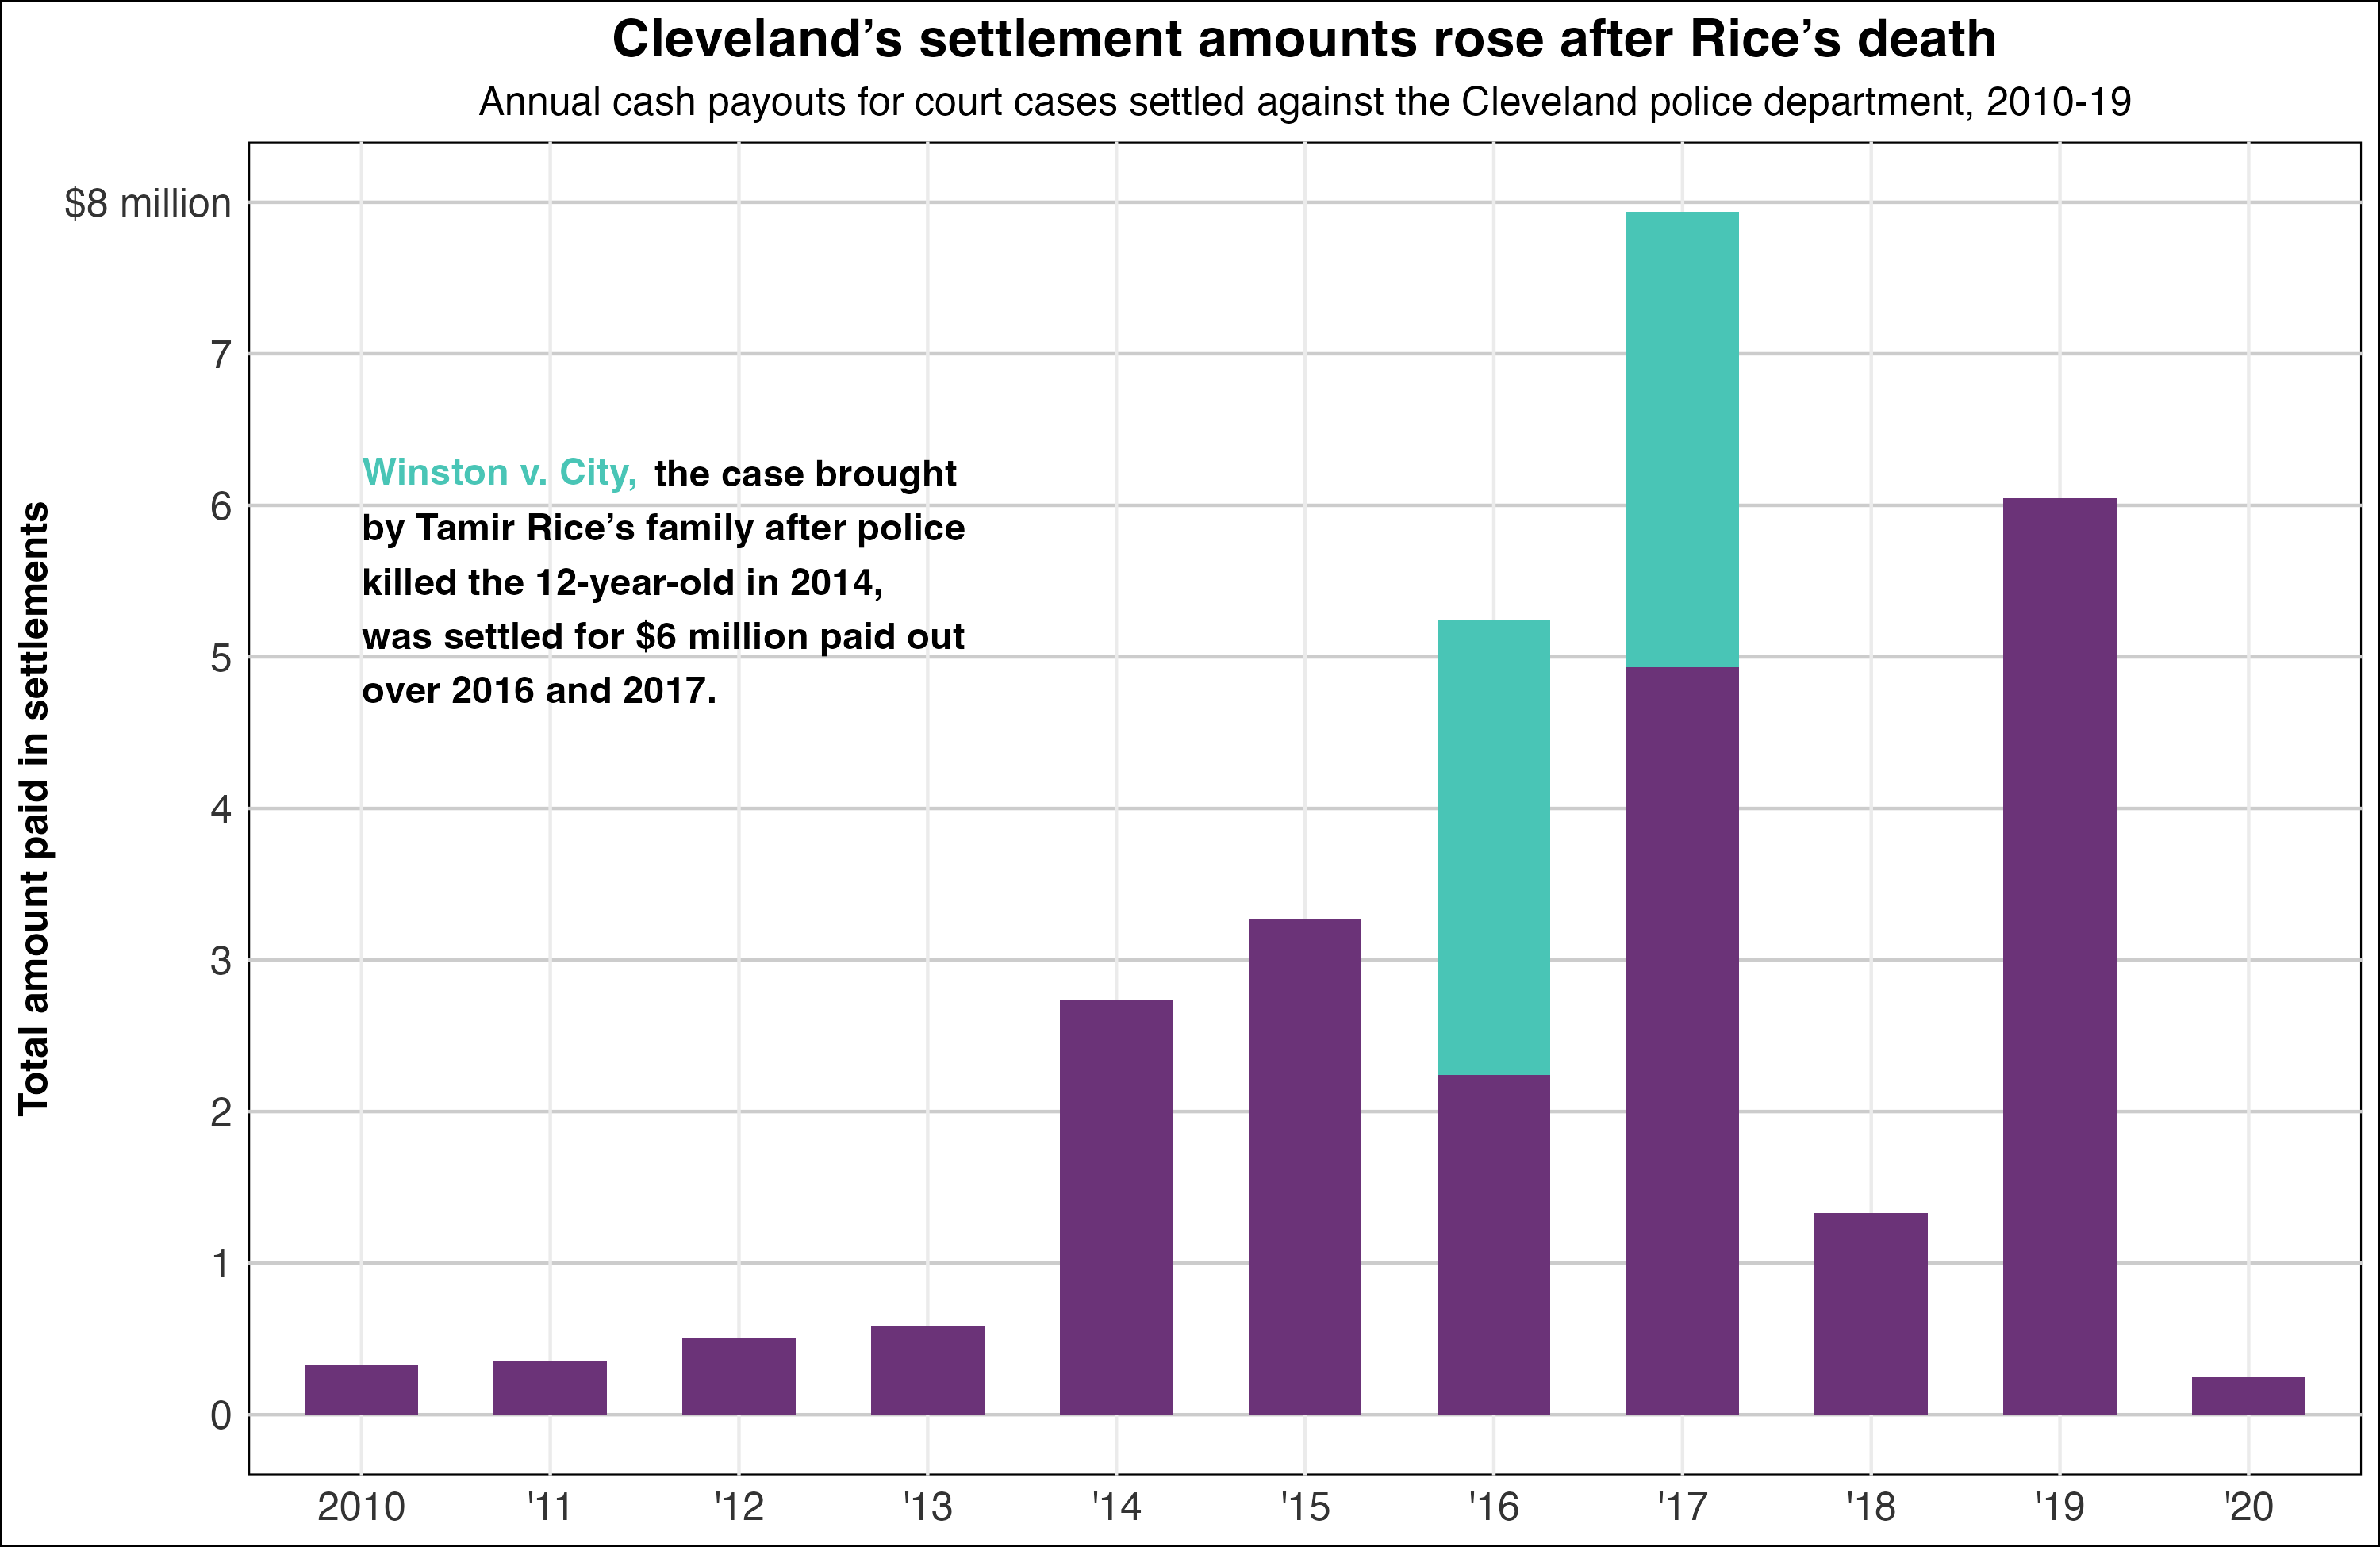
\includegraphics[width=0.6\textwidth,height=\textheight]{plots/Figure1_output.png}

From the visualization we see that the size of the bars appears to be
consistent with what is represented in the original article, and thus
the authors provided the necessary information to reproduce the figure.
Note that as described in the original article, the Cleveland Police
Department from which the data was originally collected from did not
convey descriptions of the misconduct that led to the settlements shown
above, so there may be other cases that vary in severity still included
in the annual totals, such as `payments for car accidents' (example
described from article).

\subsection{Step 3. Figure 2: Comparison of allegations between
Cincinnati versus Charleston: `Data categorization can be
misleading'}\label{step-3.-figure-2-comparison-of-allegations-between-cincinnati-versus-charleston-data-categorization-can-be-misleading}

This figure represents discrepancies and cautions readers from comparing
data from police departments of different states due to their
differences in categorization of the corresponding allegations for the
settlements. Using the final files for Cincinnati and Charleston shared
by the authors of the FiveThirtyEight article, who had processed the
data provided from their respective city police departments, we loaded
those tables and are sourcing the code with stacked barplot visual
below. The authros described that for Cincinnati cases closed between
2010-2020, some of the allegation categorization were ambiguous, with
labels like `litigation' and `negligence'. For the Charleston dataset,
the authors stated that they received PDFs from 2010-2019, a slightly
different time frame, and manually transferred some of the data with
``Law Enforcement'' within the label. The manual transferring of the
data is a bit concerning for the possibility of errors, and
additionally, the authors have noted that for this dataset there is
uncertainty of whether the data includes both claims and settlements.
The corresponding data dictionaries are listed for
\href{'https://github.com/fivethirtyeight/police-settlements/tree/main/cincinnati_oh'}{Cincinnati,
OH} and
\href{'https://github.com/fivethirtyeight/police-settlements/tree/main/charleston_sc'}{Charleston,
SC}, respectively.

\begin{Shaded}
\begin{Highlighting}[]
\FunctionTok{source}\NormalTok{(here}\SpecialCharTok{::}\FunctionTok{here}\NormalTok{(}\StringTok{\textquotesingle{}helper\_functions/Figure2\_cincinnati\_vs\_charleston.R\textquotesingle{}}\NormalTok{))}
\NormalTok{F2 }\OtherTok{\textless{}{-}} \FunctionTok{figure2}\NormalTok{(cincinnati, charleston)}
\FunctionTok{ggsave}\NormalTok{(}\AttributeTok{filename =}\NormalTok{ here}\SpecialCharTok{::}\FunctionTok{here}\NormalTok{(}\StringTok{\textquotesingle{}plots/\textquotesingle{}}\NormalTok{, }\StringTok{"Figure2\_output\_barplot.png"}\NormalTok{),}
       \AttributeTok{plot =}\NormalTok{ F2, }
       \AttributeTok{bg =} \StringTok{"white"}\NormalTok{, }\AttributeTok{width =} \DecValTok{12}\NormalTok{, }\AttributeTok{height =} \DecValTok{8}\NormalTok{, }\AttributeTok{units =} \StringTok{"in"}\NormalTok{)}

\NormalTok{knitr}\SpecialCharTok{::}\FunctionTok{include\_graphics}\NormalTok{(here}\SpecialCharTok{::}\FunctionTok{here}\NormalTok{(}\StringTok{"plots"}\NormalTok{, }\StringTok{"Figure2\_output\_barplot.png"}\NormalTok{))}
\end{Highlighting}
\end{Shaded}

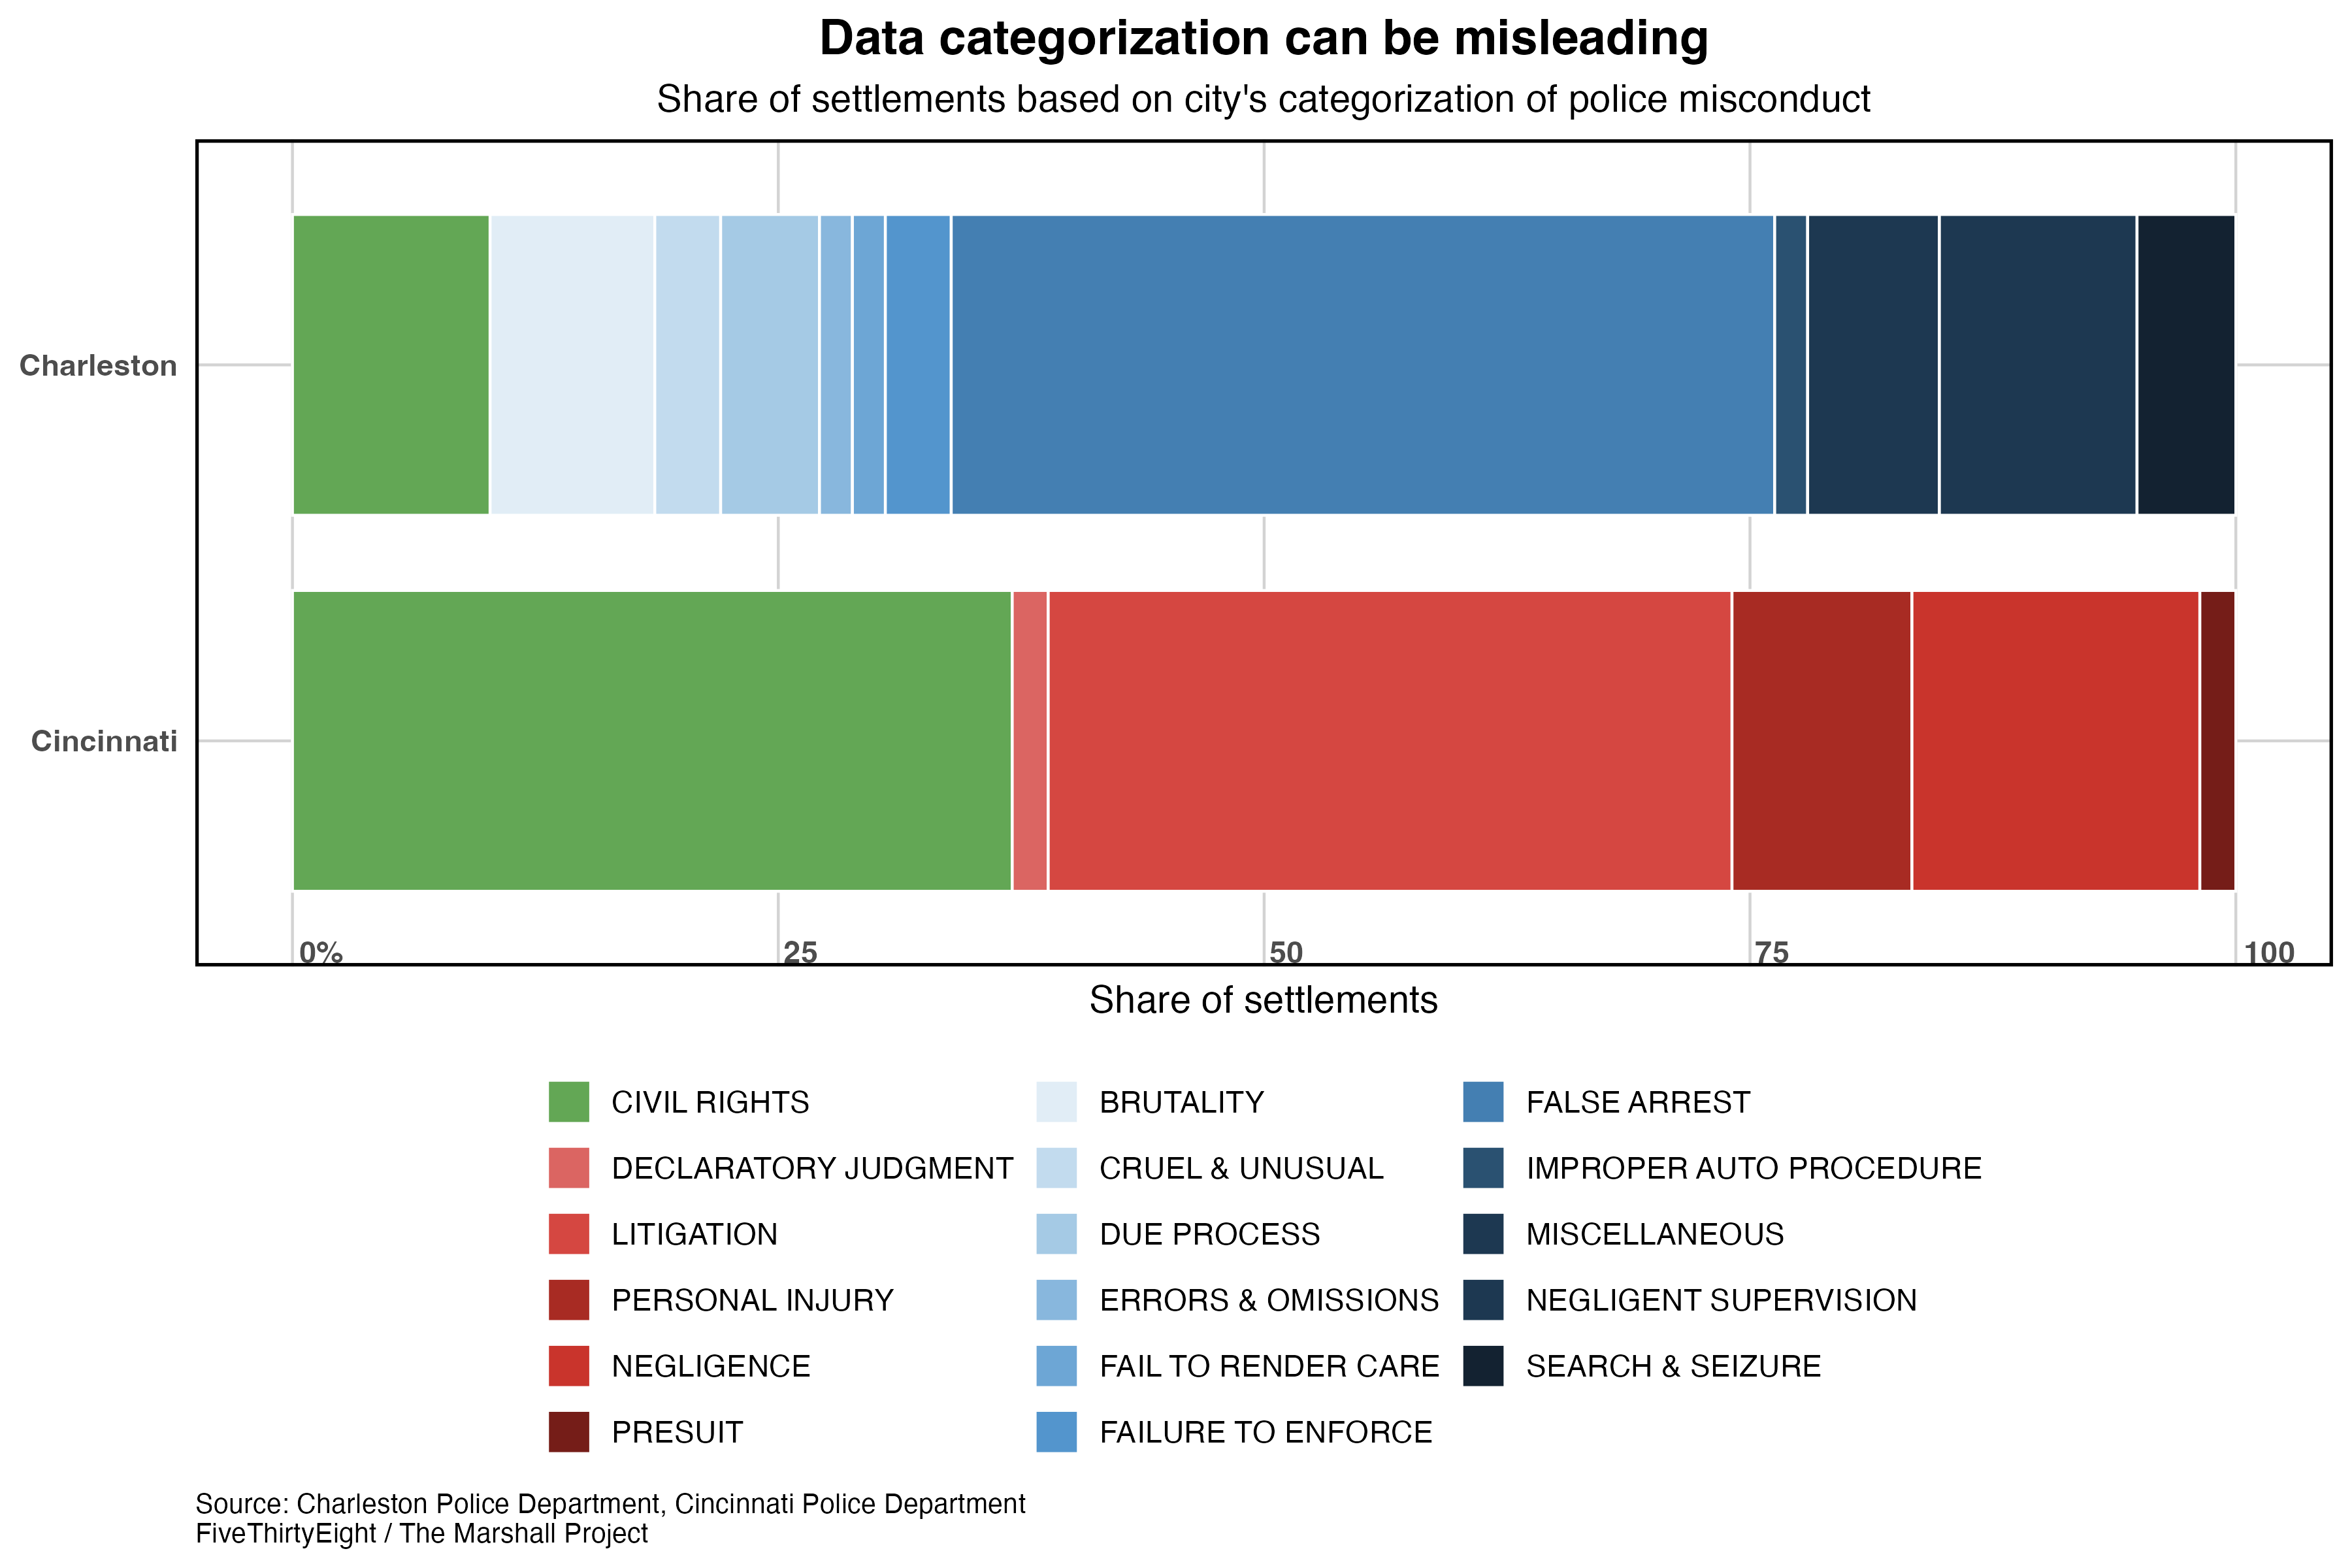
\includegraphics[width=0.6\textwidth,height=\textheight]{plots/Figure2_output_barplot.png}

The plot was not entirely reproduced the same way, including differences
in the aesthetic additions in the original image, such as captioning the
comparison between Charleston and Cincinnati that says that by the
length of the bar it appears that Cincinnati would have more civil
rights. Additionally the grouping of the legend variables. However,
using geom\_bar(stat = ``count'', position = ``fill'') parameters
allowed full expansion such that the settlement categories altogether
covered 100\%, and each of the bars and their sizes visually appear
similar to the original image. As the authors described how they
filtered the data and it was clear that the visualized stacked variable
was summary\_allegations, which are colored similarly as described to
the legend, quantitatively the figure represents the same information.
However, the final plot we have generated does not bring attention to
the categories that are only found in one of the cities versus both of
the cities as the original figure does, and as the authors noted in the
paper that the naming and sub-classifications or detailed levels in each
city varied. The percentages were also added using a manual annotation
tool to equally space out the quarter percentages and it is unclear how
these visuals were made if done in R, as this code has not been provided
by the authors.

\subsection{Step 4. Figure 3: Comparison of average and median incomes
per city in
study}\label{step-4.-figure-3-comparison-of-average-and-median-incomes-per-city-in-study}

The last figure that was attempted to be reproduced was the final figure
of the article, labeled ``Large settlements can skew a city's average
payment''. The final processed data collected from 31 city police
departments was loaded (obtained from FiveThirtyEight's GitHub), and the
corresponding csv names are stored in city\_info. As the article states,
the authors asked for detailed information of data dictionaries in the
public record requests (conducted in partnership between FiveThirtyEight
and The Marshall Project), but they only received a detailed data
dictionary from New York City. The authors conveyed that there was
ambiguity in handling the multi-year totals for the calculation of
settlement amounts, as well as how Additionally, the authors left
scratching our heads about how to understand the data underneath the
multi-year totals. The authors stated that they wanted to convey that
the settlement amount (arbitrarily decided based on how dates and
settlement and misconduct categorizations were defined per each city,
and uncertainty about the completeness of records) is hard to make clear
conclusions or interpret, as we lack information of the specific
settlements, and the measures of center of the settlements may not
indicate the severity of the case.

\begin{Shaded}
\begin{Highlighting}[]
\CommentTok{\#Create dataframe of combined data from each of the cities}
\NormalTok{full }\OtherTok{\textless{}{-}} \FunctionTok{bind\_rows}\NormalTok{(springfield, milwaukee, los\_angeles, san\_francisco, washington\_dc, }
\NormalTok{                      chicago, st\_louis, baltimore, boston, cleveland, little\_rock, }
\NormalTok{                      new\_orleans, waterbury, detroit, orlando, miami, paterson, atlanta, }
\NormalTok{                      philadelphia, baton\_rouge, indianapolis, nyc, cincinnati, columbia, }
\NormalTok{                      north\_charleston, charleston, memphis, fort\_lauderdale, roanoke, }
\NormalTok{                      cambridge, richmond)}

\CommentTok{\# Combine all datasets into a single dataframe}
\FunctionTok{source}\NormalTok{(here}\SpecialCharTok{::}\FunctionTok{here}\NormalTok{(}\StringTok{\textquotesingle{}helper\_functions/Figure3\_output\_segmentplot.R\textquotesingle{}}\NormalTok{))}
\NormalTok{F3 }\OtherTok{\textless{}{-}} \FunctionTok{figure3}\NormalTok{(}\AttributeTok{all\_data =}\NormalTok{ full)}
\FunctionTok{ggsave}\NormalTok{(}\AttributeTok{filename =}\NormalTok{ here}\SpecialCharTok{::}\FunctionTok{here}\NormalTok{(}\StringTok{\textquotesingle{}plots/\textquotesingle{}}\NormalTok{, }\StringTok{"Figure3\_output\_segmentplot.png"}\NormalTok{),}
       \AttributeTok{plot =}\NormalTok{ F3, }
       \AttributeTok{bg =} \StringTok{"white"}\NormalTok{, }\AttributeTok{width =} \DecValTok{9}\NormalTok{, }\AttributeTok{height =} \DecValTok{13}\NormalTok{, }\AttributeTok{units =} \StringTok{"in"}\NormalTok{)}

\NormalTok{knitr}\SpecialCharTok{::}\FunctionTok{include\_graphics}\NormalTok{(here}\SpecialCharTok{::}\FunctionTok{here}\NormalTok{(}\StringTok{"plots"}\NormalTok{, }\StringTok{"Figure3\_output\_segmentplot.png"}\NormalTok{))}
\end{Highlighting}
\end{Shaded}

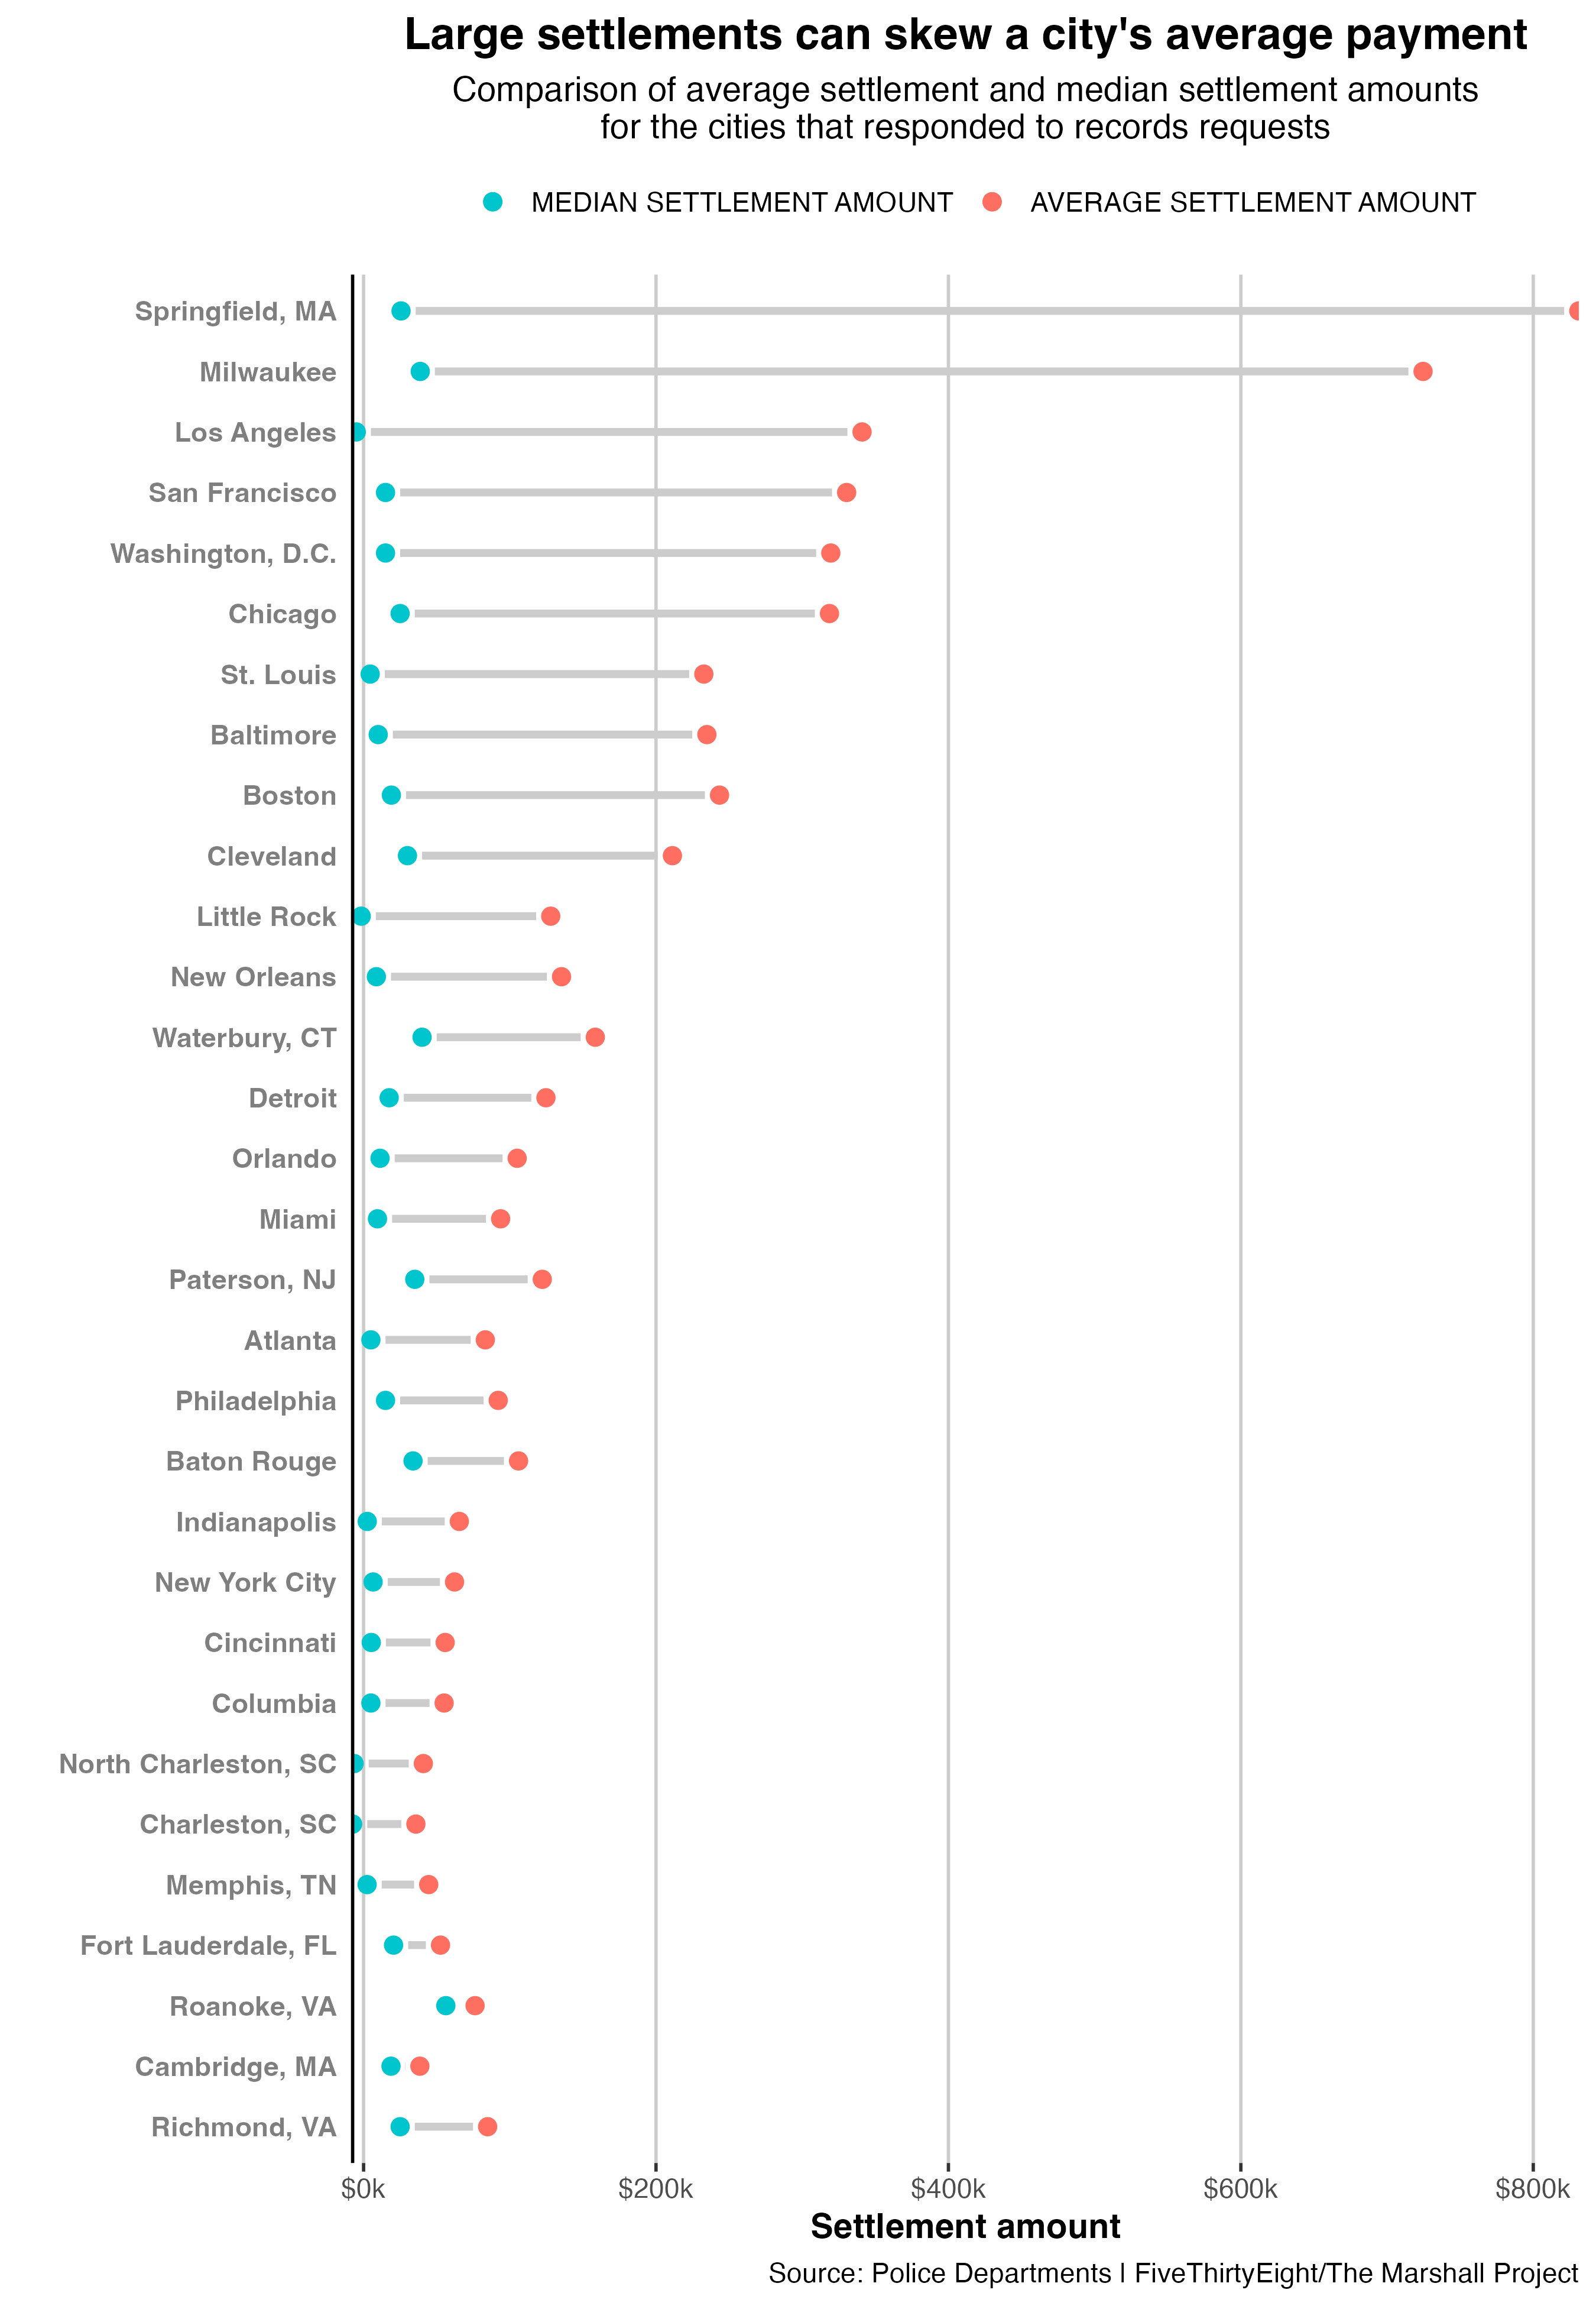
\includegraphics[width=0.6\textwidth,height=\textheight]{plots/Figure3_output_segmentplot.png}

Overall, the authors did provide several aspects included multiple
levels of the data files and processing steps, as well as a data
dictionary, which were extremely helpful for reproducing the figures.
The authors were able to provide the data that they collected publicly
from each of the city police departments and convey inconsistencies as
well as missing information for any of the fields and changes over the
approximately 10 year period. Uncertainty about updates regarding
categorization or inclusion of certain cases after follow up aligns with
what the authors stated about their conclusion that it is not advisable
to compare different cities police settlement data, since each city
conducts their record keeping differently. Additionally, there could be
more standardization of data fields across regions to help with
comparisons across and within cities over time. However, overall, the
data was accessible, codes for any formatting were generally explained
or provided, and some visualizations slightly differed based on tools
which were used (which were not shared) however appeared to convey
similar information.

\subsection{Appendix. Session Info}\label{appendix.-session-info}

\begin{Shaded}
\begin{Highlighting}[]
\FunctionTok{sessionInfo}\NormalTok{()}
\end{Highlighting}
\end{Shaded}

\begin{verbatim}
R version 4.4.2 (2024-10-31)
Platform: aarch64-apple-darwin20
Running under: macOS Sonoma 14.5

Matrix products: default
BLAS:   /Library/Frameworks/R.framework/Versions/4.4-arm64/Resources/lib/libRblas.0.dylib 
LAPACK: /Library/Frameworks/R.framework/Versions/4.4-arm64/Resources/lib/libRlapack.dylib;  LAPACK version 3.12.0

locale:
[1] en_US.UTF-8/en_US.UTF-8/en_US.UTF-8/C/en_US.UTF-8/en_US.UTF-8

time zone: America/New_York
tzcode source: internal

attached base packages:
[1] stats     graphics  grDevices utils     datasets  methods   base     

other attached packages:
[1] scales_1.3.0    tinytex_0.54    ggplot2_3.5.1   stringr_1.5.1  
[5] lubridate_1.9.4 dplyr_1.1.4     tidyr_1.3.1     here_1.0.1     
[9] readxl_1.4.3   

loaded via a namespace (and not attached):
 [1] gtable_0.3.6      jsonlite_1.8.9    compiler_4.4.2    tidyselect_1.2.1 
 [5] textshaping_0.4.1 systemfonts_1.1.0 yaml_2.3.10       fastmap_1.2.0    
 [9] R6_2.5.1          labeling_0.4.3    generics_0.1.3    knitr_1.49       
[13] tibble_3.2.1      munsell_0.5.1     rprojroot_2.0.4   pillar_1.10.1    
[17] rlang_1.1.4       stringi_1.8.4     xfun_0.50         timechange_0.3.0 
[21] cli_3.6.3         withr_3.0.2       magrittr_2.0.3    digest_0.6.37    
[25] grid_4.4.2        rstudioapi_0.17.1 lifecycle_1.0.4   vctrs_0.6.5      
[29] evaluate_1.0.1    glue_1.8.0        farver_2.1.2      cellranger_1.1.0 
[33] ragg_1.3.3        colorspace_2.1-1  rmarkdown_2.29    purrr_1.0.2      
[37] tools_4.4.2       pkgconfig_2.0.3   htmltools_0.5.8.1
\end{verbatim}




\end{document}
